\documentclass[10pt,psamsfonts,reqno,oneside,letterpaper]{amsart}
\usepackage[dvips,text={6.5truein,9truein},left=1truein,top=1truein]{geometry}
\usepackage{amssymb,amsmath,amscd,enumerate}
\usepackage{amscd}
\usepackage[pdftex]{graphicx}
\usepackage{graphicx}
\usepackage{caption}
\usepackage{subcaption}
\usepackage[colorlinks,linkcolor=black,citecolor=black,pdfstartview=FitH]{hyperref}
\usepackage{pgfplots}
\usetikzlibrary{calc}

% Uncomment to use syncing

%\usepackage{pdfsync}


% Paragraphs
\parindent=0pt
\parskip=5 pt plus 2 pt minus 1pt

%color shortcuts
\usepackage{color}
\newcommand\change[1]{{\color{red}#1}}
\newcommand\delete[1]{{\color{green}#1}}
\newcommand\comment[1]{{\color{blue}#1\color{black}}}

\newcommand{\xdownarrow}[1]{%
	{\left\downarrow\vbox to #1{}\right.\kern-\nulldelimiterspace}
}

\newtheorem{theorem}{Theorem}
\newtheorem{corollary}{Corollary}
\newtheorem{definition}{Definition}
\newtheorem{proposition}{Proposition}
\newtheorem{lemma}{Lemma}

%other shortcuts
\newcommand\Z{{\mathbb Z}}
\newcommand\N{{\mathbb N}}
\newcommand\C{{\mathbb C}}
\newcommand\Q{{\mathbb Q}}
\newcommand\R{{\mathbb R}}
\newcommand\id{{\mathrm{id}}}
\newcommand\im{{\mathrm{im}}}

\begin{document}
	
	
	\section*{Math 18500 - Problem Set 5}
	\begin{enumerate}[I]

\item Find the general solution of each of the following second order inhomogeneous equations:
\begin{enumerate}
	\item  $y'' + 3y' + 2y = e^{2t}$
	\item  $y'' + 3y' + 2y = e^{-2t}$
	\item  $y'' + 4y' + 4y = e^{-2t} $
\end{enumerate}

\item  Find a particular solution of the equation
\[ y'' + 3y' + 2y = \cos t + 2\sin t \]
and write it in each of the following forms:
\begin{enumerate}
	\item  $y = \mathrm{Re}\left[ Z e^{i\omega t} \right] $ where $\omega>0$ and $Z$ is a complex number.
	\item  $y = a \cos(\omega t) + b \sin(\omega t)$ where $\omega>0$ and $a$ and $b$ are real numbers.
	\item  $y = A \cos(\omega  t - \phi)$ where $A>0$, $\omega>0$, and $0 \leq \phi < 2\pi$.
\end{enumerate}

\item  Solve the following initial value problem:
\[ y'' + 3y' + 2y =  5e^{2t} + 6e^{-2t} + 3\cos(t) + 6\sin(t)  \; , \; \; y(0) = 1 \;, \; \; y'(0) = 1 \]
\textit{Hint: Use the work you did in problems 1 and 2!}

\item  Consider a general second order equation of the form
\[ (D-\lambda_1)(D-\lambda_2) y = e^{\lambda_1 t} \]
where $\lambda_1$ and $\lambda_2$ are arbitrary constants.
\begin{enumerate}
	\item  If $\lambda_1 \neq \lambda_2$, the method of undetermined coefficients says to guess a particular solution of the form 
	\[ y = At e^{\lambda_1 t}. \]
	for some value of $A$.  This leads to a general solution of the form 
	\[ y = A t e^{\lambda_1 t} + B e^{\lambda_1 t} + Ce^{\lambda_2 t}. \]
	Justify this ``lucky guess'' using the repeated integration method.
	\item  If $\lambda_1 = \lambda_2$, the method of undetermined coefficients says to guess a particular solution of the form 
	\[ y = At^2 e^{\lambda_1 t} \]
	for some value of $A$.  This leads to a general solution of the form
	\[ y = At^2 e^{\lambda_1 t}+ B te^{\lambda_1 t} + Ce^{\lambda_1 t}. \]
	Justify this ``lucky guess'' using the repeated integration method.
\end{enumerate}

\item  Consider a fluid-filled box which contains a solid block attached to the ends of the box with two identical springs:
\[ 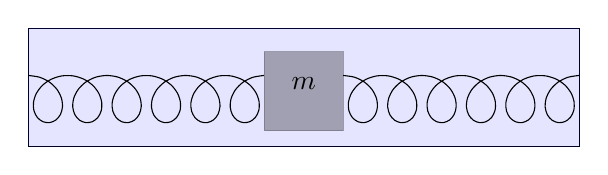
\begin{tikzpicture}
	\draw[solid] (0,1)--(0,-0.5)--(7,-0.5)--(7,1)--(0,1);
	\draw[fill,blue,opacity=0.1] (0,1)--(0,-0.5)--(7,-0.5)--(7,1)--(0,1);
	\draw[variable=\x,domain=0:3, smooth, samples=100] plot(({\x + 0.3*sin(720*\x)},{0.1+0.3*cos(720*\x)});
	\draw[fill,opacity=0.3] (3,-0.3)--(3,0.7)--(4,0.7)--(4,-0.3)--(3,-0.3);
	\node at (3.5,0.3) {$m$};
	\draw[variable=\x,domain=0:3, smooth, samples=100] plot(({4+\x + 0.3*sin(720*\x)},{0.1+0.3*cos(720*\x)});
\end{tikzpicture}
\] 
Let $y$ denote the displacement of the block from the center of the box (so in the picture above, $y=0$).  Then the motion of the block can be modelled using an equation of the form
\[ my'' + l y' + k y = f(t), \]
where $m>0$ represents the mass of the block, $k>0$ represents the tightness of the spring, $l>0$ represents the stickiness (\textit{viscosity}) of the fluid, and $f(t)$ represents the sum of all external forces acting on the block.  Assume that the mass of the block is $1$ kilogram.
\begin{enumerate}
	\item  You suddenly turn the box on its side, like this:
	\[ 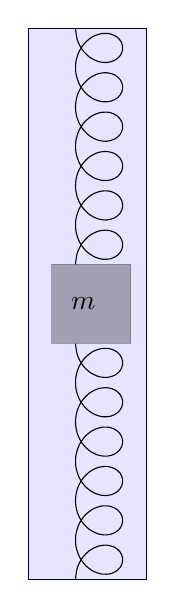
\begin{tikzpicture}[rotate=90]
		\draw[solid] (0,1)--(0,-0.5)--(7,-0.5)--(7,1)--(0,1);
		\draw[fill,blue,opacity=0.1] (0,1)--(0,-0.5)--(7,-0.5)--(7,1)--(0,1);
		\draw[variable=\x,domain=0:3, smooth, samples=100] plot(({\x + 0.3*sin(720*\x)},{0.1+0.3*cos(720*\x)});
		\draw[fill,opacity=0.3] (3,-0.3)--(3,0.7)--(4,0.7)--(4,-0.3)--(3,-0.3);
		\node at (3.5,0.3) {$m$};
		\draw[variable=\x,domain=0:3, smooth, samples=100] plot(({4+\x + 0.3*sin(720*\x)},{0.1+0.3*cos(720*\x)});
	\end{tikzpicture}
	\] 
	Now block is subject to the force of gravity, and its motion can be modeled by solving the initial value problem
	\[ my'' + ly' + ky = - mg \; , \; \; y(0) = 0 \; , \; \; y'(0) = 0, \]
	where $g \approx 10 \textrm{ meters/second}^2$.   If the block comes to rest $10$ centimeters below its original equilibrium position, determine the value of $k$ (in units of kilograms/second$^2$).
	\item As the block comes to rest, it oscillates around its new equilibrium position (10 centimeters below its original equilibrium position).  Using a high speed camera, you measure the times at which the object passes through its new equilibrium position, and find this is happenening once per second.  Based on this experiment, and your answer to part \textbf{a}, determine the value of $l$ (in units of kilograms/second).
\end{enumerate}
\item  Consider a similar box to the one described in problem 5, but assume the values $m = k = 1$.  Instead of turning the box on its side, you gently rock it back and forth at a constant frequency.  Now the motion of the block can be modeled by solving the initial value problem 
\[ y'' + ly' + y = A_d \cos(\omega_d t) \; , \; \; y(0) = 0 \; , \; \; y'(0) = 0. \]
where $\omega_d$ and $A_d$ are positive constants (the \emph{driving frequency} and \emph{driving amplitude}).
\begin{enumerate}
	\item  Show that the solution takes the form
	\[ y = A \cos(\omega_d t - \phi) + y_h(t) \]
	where $A$ and $\phi$ are positive constants and $y_h(t)$ is a solution of the homogeneous equation
	\[ y'' + ly' + y = 0. \]
	Give explicit formulas for $A$ and $\phi$ in terms of $A_d$, $\omega_d$, and $l$.
	\item Note that $\displaystyle \lim_{t \to \infty} y_h(t) = 0$ for any value of $l$.  Because of this, $y_h(t)$ is often referred to as a \emph{transient}.  As you increase the value of $l$, does the transient die off more or less rapidly?
	\item  The ratio $A/A_d$ is called the \emph{amplitude gain} of the system.  Using a computer, plot the amplitude gain as a function of $\omega$, for a few different values of $l$:
	\[ l = 0.01, 0.1, 1, 10, 100 \]
	\item  Let $\omega_r$ be the value of the driving frequency which results in the maximum amplitude gain (the \emph{resonant frequency}). Give a formula for $\omega_r$ as a function of $l$, assuming that $l$ is small and positive.  Is it greater or less than the natural frequency $\omega_0$?  (\textit{See problem set 4 for the definition of $\omega_0$})
	\item  If the value of $l$ is sufficiently large, then the resonant frequency will be $0$.  Give a formula for the smallest value of $l$ such that this occurs.   Is it greater than, less than, or equal to the value of $l$ at which critical damping occurs?
	\item   What is the solution of the initial value problem if $l = 0$ and $\omega_d = \omega_r$? Plot it as a function of $t$. 
\end{enumerate}
	\end{enumerate}
	
	
	

\end{document} 




